\documentclass[12pt]{exam}
% \documentclass[12t, answers]{exam}
\usepackage[portuguese]{babel}
\usepackage[utf8]{inputenc}
\usepackage{graphicx}
\graphicspath{{figuras/}}
\usepackage{amssymb}
\usepackage[margin=1in]{geometry}
\usepackage{enumerate}% http://ctan.org/pkg/enumerate
\usepackage{amsmath,amssymb}
\usepackage{multicol}
\usepackage{textcomp,lmodern,listings}
\usepackage{xcolor}
% Definindo novas cores
\definecolor{verde}{rgb}{0.25,0.5,0.35}
\definecolor{jpurple}{rgb}{0.5,0,0.35}
% Configurando layout para mostrar codigos Java
\usepackage{listings}
\lstset{
	language=Java,
	basicstyle=\ttfamily\small, 
%	keywordstyle=\color{jpurple}\bfseries,
%	stringstyle=\color{red},
	commentstyle=\color{verde},
	morecomment=[s][\color{blue}]{/**}{*/},
	extendedchars=true, 
	showspaces=false, 
	showstringspaces=false, 
	numbers=left,
	numberstyle=\tiny,
	breaklines=true, 
%	backgroundcolor=\color{cyan!10}, 
	breakautoindent=true, 
	captionpos=b,
	xleftmargin=0pt,
	tabsize=3
}
\newcommand{\disciplina}{Banco de Dados}
\newcommand{\class}{\disciplina}
\newcommand{\term}{Prof. Dr. Igor Avila Pereira}
\newcommand{\bimestre}{}
\newcommand{\valor}{10}
\newcommand{\examnum}{Exame -- Valor: \valor}
%\newcommand{\examdate}{xx}
%\newcommand{\timelimit}{4 horas}

\pagestyle{head}
\firstpageheader{}{}{}
\runningheader{\class} - {Página \thepage\ de \numpages}
\runningheadrule

% https://math.mit.edu/~psh/exam/examdoc.pdf
% caixinha em vez de bolinha
\checkboxchar{$\Box$}
% reposta com caixinha preta em vez de checked
\checkedchar{$\blacksquare$}
% mostrar as respostas (gabarito)
\printanswers

% trocar a palavra point(s) por nada
\pointname{}
% https://groups.google.com/g/latex-br/c/DHdjfnfN90M

%\bonuspointpoins{ponto (bônus)}{pontos (bônus)}

\begin{document}

\noindent
\begin{tabular*}{\textwidth}{l @{\extracolsep{\fill}} r @{\extracolsep{6pt}} l}
\textbf{\class} & \textbf{Nome:} & \makebox[2in]{\hrulefill}   \\
\textbf{\examnum} & \textbf{Matrícula:} & \makebox[2in]{\hrulefill}   \\
%\textbf{\examnum} &&\\
%\textbf{\examdate} &&\\
\textbf{\term} &&\\
%\textbf{Duração: \timelimit}
\end{tabular*}\\
\rule[2ex]{\textwidth}{2pt}
\noindent
%rule[2ex]{\textwidth}{2pt}

\begin{questions}

\question[0.5] Uma entidade que não tem atributos suficientes para formar um atributo identificador é denominada:

\begin{checkboxes}
\choice mole.
\choice vazia.
\choice secundária.
\CorrectChoice fraca.
\choice normal.
\end{checkboxes}

%\textbf{Gabarito: Fraca}

\question[0.5] Os atributos que podem ser divididos em subpartes menores e que representam atributos mais básicos, com significados independentes, são considerados atributos:

\begin{checkboxes}
\choice atômicos.
\CorrectChoice compostos.
\choice multivalorados.
\choice complexos.
\choice derivados.
\end{checkboxes}

%\textbf{Gabarito: composto}

\question[0.5] Analise a figura abaixo:

\begin{figure}[!htp]
\centering
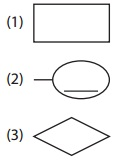
\includegraphics[width=0.2\linewidth]{figuras/57_QUESTAO}
%\caption{}
\label{fig:57_QUESTAO}
\end{figure}

Assinale a alternativa que corresponde corretamente à sequência das notações do Diagrama Entidade-Relacionamento (DER) acima.

\begin{checkboxes}
\choice (1) Relacionamento; (2) Atributo Chave; (3) Entidade.
\CorrectChoice (1) Entidade; (2) Atributo Chave; (3) Relacionamento.
\choice (1) Entidade; (2) Atributo Derivado; (3) Relacionamento.
\choice (1) Composto; (2) Atributo Chave; (3) Relacionamento.
\choice (1) Entidade; (2) Atributo Composto; (3) Relacionamento.
\end{checkboxes}	

%\textbf{Gabarito:  (1) Entidade; (2) Atributo Chave; (3) Relacionamento.}

% \newpage

\question[0.5] Assinale a opção que descreve o tipo de atributo previsto no modelo ER que não precisa ser obrigatoriamente, armazenado no banco de dados: 

\begin{checkboxes}
\choice Composto.
\choice Multivalorado.
\choice Nulo.
\CorrectChoice Derivado.
\choice Simples.
\end{checkboxes}

%\textbf{Gabarito: derivado}

\question[0.5] Considere o seguinte diagrama entidade-relacionamento de um banco de dados relacional, representando as bibliotecas de uma universidade.

\begin{figure}[!htp]
\centering
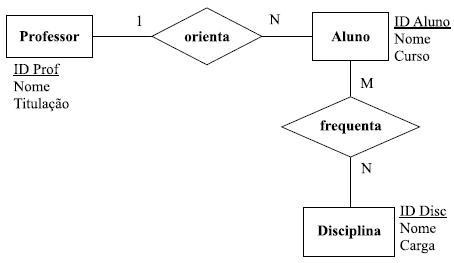
\includegraphics[width=0.7\linewidth]{figuras/Imagem004}
%\caption{}
\label{fig:Imagem004}
\end{figure}

A partir desse diagrama, pode-se afirmar que

\begin{checkboxes}
\choice Aluno e Disciplina são entidades fracas.
\choice Disciplina não pode ter atributos com o valor nulo.
\CorrectChoice um aluno pode frequentar diversas disciplinas e pode ser orientado por apenas um professor.
\choice os atributos ID Prof, ID Aluno e ID Disc devem ser implementados como sendo do tipo literal.
\choice todos os atributos de Aluno podem ser classificados como compostos.
\end{checkboxes}

%\textbf{Gabarito:  um aluno pode frequentar diversas disciplinas e pode ser orientado por apenas um professor.}

% \newpage

\question[0.5] Observe o banco de dados composto pelas relações a seguir, em que atributos sublinhados indicam a chave primária, e atributos em itálico apontam as chaves estrangeiras.

\begin{itemize}
    \item funcionário(\underline{NrMatric}, NmFunc, DtAdmin, Sexo, \textit{CdCargo}, \textit{CdDepto})
    \item cargo (\underline{CdCargo}, NmCargo, ValorSalario)
    \item departamento (\underline{CdDepto}, NmDepto, Ramal)
\end{itemize}

% \begin{figure}[!htp]
% \centering
% 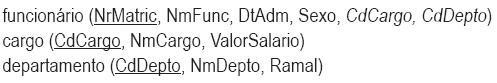
\includegraphics[width=0.7\linewidth]{figuras/Imagem017}
% %\caption{}
% \label{fig:Imagem017}
% \end{figure}

\newpage

Com base nisso, pode-se afirmar que:

\begin{enumerate}[I]	
\item - um funcionário está alocado em um departamento; 
\item - podem existir valores nulos para o atributo NrMatric; 
\item - pode haver mais de um departamento com o mesmo ramal; 
\item - um funcionário possui um cargo; 
\item - pode haver mais de um cargo com o mesmo ValorSalario.
\end{enumerate}

São corretas APENAS as afirmações:

\begin{checkboxes}
\choice II e III.
\choice IV e V.
\choice I, III e IV.
\choice II, IV e V.
\CorrectChoice I, III, IV e V.
\end{checkboxes}

%\textbf{Gabarito:  I, III, IV e V.}

% \question[0.5] Como passamos por Spark um parâmetro por GET?

% \begin{checkboxes}
% \choice /rota/igor
% \choice /rota?parametro=igor
% \choice /rota?igor
% \choice /rota=igor
% \choice /igor
% \end{checkboxes}

%\textbf{Gabarito: /rota/igor}

% \question[0.5] Qual função que redireciona entre rotas no Spark?


% \begin{checkboxes}
% 	\choice redirect("/rota");
% 	\choice this.redirect("/rota");
% 	\choice response.url("/rota");
% 	\choice request.redirect("/rota");
% \choice response.redirect("/rota");
% 	\end{checkboxes}
	
%	\textbf{Gabarito: response.redirect("/rota");}

% \newpage

%\question[0.5]  Na linguagem SQL, a consulta simples a um Banco de Dados é uma instrução SELECT e a consulta composta inclui duas ou mais instruções SELECT. Com relação às consultas com a utilização da linguagem SQL é correto afirmar que o operador
%
%\begin{checkboxes}
%	\choice UNION é usado para combinar os resultados de duas ou mais instruções SELECT, retornando linhas duplicadas.
%	\choice UNION ALL, quando usado na combinação de duas instruções SELECT, a ordem das instruções SELECT altera o resultado da consulta.
%	\choice EXCEPT, quando usado na combinação duas instruções SELECT, a ordem das instruções SELECT não altera o resultado da consulta.
%	\choice EXCEPT é usado para combinar duas ou mais instruções SELECT, retornando somente as linhas da primeira instrução SELECT que sejam semelhantes a uma linha das demais instruções.
%	\choice INTERSECT é usado para combinar duas instruções SELECT, retornando somente as linhas da primeira instrução SELECT que sejam idênticas a uma linha da segunda instrução SELECT.
%\end{checkboxes}

% \question[0.5] No Java, a classe \textit{DriverManager} fornece os serviços básicos para gerenciamento de drivers JDBC. Quais três argumentos normalmente são passados como parâmetros em seu método \textit{getConnection}? 

% \begin{checkboxes}
% 	\choice String url, String user e String password.
% 	\choice String url, String port e String database.
% 	\choice String url, String user e String database. 
% 	\choice String user, String port e String database.
% 	\choice String user, String password e String database. 
% \end{checkboxes}

%\textbf{Gabarito: String url, String user e String password.}

% \question[0.5] Analise o código a seguir.

% \vspace{20px}

% \begin{lstlisting}
% import java.sql.*;
% public class Dao {
% 	public int metodoA(String v) {
% 		int x = 0;
% 		try {
% 			Class.forName("com.mysql.jdbc.Driver");
% 			Connection con = DriverManager.getConnection
% 			("jdbc:mysql://localhost:3306/controle", "root", "x");
% 			Statement st = con.createStatement();
% 			x = st.executeUpdate(v);
% 			return x;
% 		} catch (ClassNotFoundException ex) {
% 			return x;
% 		} catch (Exception ex1) {
% 			return x;
% 		}
% 	}
% }
% \end{lstlisting}

% \vspace{20px}

% Para que o metodoA execute a operação desejada, na chamada ao método executeUpdate é necessário que ele receba como parâmetro uma instrução DML SQL

% \begin{checkboxes}
% 	\choice update, apenas.
% 	\choice insert, update, delete ou select.
% 	\choice insert, update ou delete, apenas.
% 	\choice insert, apenas.
% 	\choice update ou select, apenas.
% \end{checkboxes}

%\textbf{Gabarito: insert, update ou delete, apenas.}

% \newpage

% \question[0.5] Nas classes, nas quais estes métodos se encontram, foram importados todos os recursos necessários para a execução. O banco de dados, a tabela e o driver JDBC existem e funcionam corretamente. 

% \vspace{20px}

% \textbf{Método 1}

% \vspace{15px}


% \begin{lstlisting}
% public int inserir(int varId, String varNome, double varRenda){
% 	int retorno;
% 	try {
% 		Class.forName("com.mysql.jdbc.Driver");
% 		Connection conn = DriverManager.getConnection("jdbc:mysql://localhost:3306/bd007", "root", "1234");
% 		PrepareStatement st = conn.prepareStatement("insert into cliente (id, nome, renda) values (?,?,?);");
% 		st.setInt(1, varId);
% 		st.setString(2, varNome);
% 		st.setDouble(3, varRenda);
% 		retorno = st.executeUpdate();
% 	} catch (ClassNotFoundException ex){
% 		retorno = 0;		
% 	} catch (SQLException ex1){
% 		retorno = 0;
% 	}
% 	return retorno;
% }
% \end{lstlisting}

% \vspace{20px}

% \textbf{Método 2}

% \vspace{15px}

% \begin{lstlisting}
% public int inserir (int varId, String varNome, double varRenda){
% 	int retorno;
% 	try {
% 		Class.forName("com.mysql.jdbc.Driver");
% 		Connection conn =  DriverManager.getConnection("jdbc:mysql://localhost:3306/bd007","root","1234");
% 		Statement st = conn.createStatement();
% 		retorno = st.executeUpdate("insert into cliente values ('"+varId+"', '"+varNome+"', "+varRenda+")");
% 	} catch (ClassNotFoundException ex){
% 		retorno = 0;		
% 	} catch (SQLException ex1){
% 		retorno = 0;
% 	}
% 	return retorno;
% }
% \end{lstlisting}

%\begin{figure}[!htp]
%	\centering
%	\includegraphics[width=0.9\linewidth]{figuras/metodo2}
%%	\caption{}
%	\label{fig:metodo2}
%\end{figure}

%\newpage

% É correto afirmar que:

% \begin{checkboxes}
% 	\choice o Método 1 está incorreto, pois o método executeUpdate da interface PreparedStatement precisa receber como parâmetro a instrução SQL insert a ser executada.
% 	\choice o Método 2 está incorreto, pois o método executeUpdate da interface Statement não pode receber parâmetros. A instrução insert passada como parâmetro nesse método deveria ser passada como parâmetro para o método createStatement da interface Connection.
% 	\choice ambos os métodos estão corretos e executam a mesma operação, apresentando os mesmos resultados.
% 	\choice ambos os métodos estão incorretos, pois o método presente tanto na interface Statement como na interface PreparedStatement para incluir dados na tabela do banco de dados é o método executeInsert e não executeUpdate .
% 	\choice o Método 1 está incorreto, pois a instrução insert passada como parâmetro para o método PreparedStatement da interface Connection está incompleta. No lugar dos pontos de interrogação devem ser colocados os valores que devem ser incluídos nos campos id , nome e renda da tabela.	
% 	\end{checkboxes}

%\textbf{Gabarito:ambos os métodos estão incorretos, pois o método presente tanto na interface Statement como na interface PreparedStatement para incluir dados na tabela do banco de dados é o método executeInsert e não executeUpdate.}

%\question[0.5] Como críamos e retornamos a sessão criada com Spark?
%
%\textbf{Gabarito:} 
%\begin{lstlisting} 
%request.session(true); // create and return session 
%\end{lstlisting}

%\question[0.5] Como faz para redirecionar entre rotas?
%
%\textbf{Gabarito:} 
%\begin{lstlisting} 
%response.redirect("/bar");
%\end{lstlisting}
%
%\question[0.5] Crie uma rota GET que dê \textit{Hello World} para o usuário.
%
%\textbf{Gabarito:} 
%\begin{lstlisting}
%import static spark.Spark.*;
%public class HelloWorld {
%	public static void main(String[] args) {
%		get("/hello", (req, res) -> "Hello World");
%	}
%}
%\end{lstlisting}
%
%\question[0.5] Como devemos percorrer uma coleção usando o MustacheTemplate? Como ficaria um \textit{ArrayList} que contém objetos da classe \textit{Pessoa}. Obs: A classe \textit{Pessoa} possui os seguintes atributos: id, nome e sobrenome.
%
%\textbf{Gabarito:} 
%\begin{lstlisting}
%<table>
%	{{#pessoas}}
%		<tr>
%			<td>{{id}}</td>  
%			<td>{{nome}}</td> 
%			<td>{{sobrenome}}</td>
%		</tr>
%	{{/pessoas}}
%</table>
%\end{lstlisting}


%\question[0.5] Como obtemos nos Commands parâmetros vindos por GET dentro do Spark?
%
%\textbf{Gabarito:} 
%\begin{lstlisting}
%request.params(":id");
%\end{lstlisting}
%
%\question[0.5] Como obtemos nos Commands parâmetros vindos por POST dentro do Spark?
%
%\textbf{Gabarito:} 
%\begin{lstlisting}
%request.queryParams("nome");
%\end{lstlisting}


%\question[0.5] Mostre os autores que seu nome comece com R e termine com O (baseado no esquema da figura \ref{fig:ER_catalogocds}).
%
%
%\textbf{Gabarito:}
%
%\begin{lstlisting}
%SELECT nome_autor FROM autor WHERE nome_autor ILIKE 'r%O';
%\end{lstlisting}
%
%\question[0.5] Mostre o nome e o codigo dos CDs da gravadora de codigo 2.
%
%\begin{lstlisting}
%SELECT nome_cd, codigo_cd
%FROM gravadora INNER JOIN cd 
%	ON (cd.codigo_gravadora=gravadora.codigo_gravadora)
%WHERE gravadora.codigo_gravadora = 2
%\end{lstlisting}

%\question[0.5] A linguagem utilizada para realizar inclusões, consultas, alterações e exclusões de dados presentes em registros é conhecida como
%
%\begin{checkboxes}
%\choice DDL.
%\choice DML.
%\choice SQL.
%\choice DCL.
%\choice OQL.
%\end{checkboxes}
%	
%	\textbf{Gabarito: DML}
	

%\newpage	
	
% \question[0.5] Considere que o Tribunal Regional do Trabalho possua em seu Banco de Dados a tabela Processos descrita abaixo. 

% \vspace{20px}

% \begin{table}[!htp]
%  	\caption{Tabela Processos }
% 		\centering    
% 		\begin{tabular}{|c|c|}
% 			\hline \textbf{Nro\underline{\hspace{0.1cm}}Processo} &  \textbf{Envolvido} \\ 
% 			\hline 1112222-12.2011.5.04.0000   &  Maria da Silva \\
% 			\hline 3336666-36.2013.5.04.0000   &  Jose dos Santos \\
% 			\hline 7779999-79.2015.5.04.0000   &  Antonio Alves \\
% 			\hline 1234567-89.2012.5.04.0000    & Jeronimo Souza  \\
% 			\hline 
% 	\end{tabular} 
% \end{table}               

% \vspace{20px}

% O comando SQL que traz todos os dados da tabela ordenados pela ordem alfabética dos nomes dos envolvidos é: 

% %\vspace{20px}

% \begin{checkboxes}
% \choice \begin{verbatim}SELECT *.* FROM Tabela_Processos ORDERED BY Envolvido;\end{verbatim}
% \choice \begin{verbatim}SELECT * FROM Tabela_Processos ORDER BY Envolvido ASCENDING;\end{verbatim}
% \choice \begin{verbatim}SELECT Nro_Processo AND Envolvido FROM Tabela_Processos 
% ORDER BY Envolvido ASC;\end{verbatim}
% \choice \begin{verbatim}SELECT (Nro_Processo, Envolvido) FROM Processos 
% ORDER BY Nome_Envolvido;\end{verbatim}
% \choice \begin{verbatim}SELECT * FROM Processos ORDER BY Envolvido ASC;\end{verbatim}
% \end{checkboxes}

% \vspace{20px}

%\textbf{Gabarito: SELECT * FROM Processos ORDER BY Envolvido ASC;}	


%\question[0.5] Considere o banco de dados relacional EMPRESA, composto de duas relações, descrito a seguir. 
%
%\vspace{10px}
%
%A relação E refere-se aos empregados, cuja o esquema é E(CPF, Nome, Salario, CPF do Supervisor, Depto), onde: CPF identifica unicamente cada empregado; CPF do Supervisor referencia o CPF do supervisor direto do empregado; Depto referencia o departamento em que o empregado está lotado; e Nome e Salário denotam o nome e o salário do empregado, respectivamente. A relação D refere-se aos departamentos, cujo esquema é D (Código, Nome), onde: Código identifica unicamente cada departamento; e Nome denota o nome do departamento. 
%
%\vspace{10px}
%
%A consulta “Qual a identificação dos departamentos, cujo número de empregados lotados é superior a 5?” ao banco de dados EMPRESA pode ser escrita em SQL segundo a expressão
%
%\begin{checkboxes}
%\choice SELECT Depto FROM E GROUP BY Depto HAVING COUNT(*) $>$ 5
%\choice SELECT Depto FROM E WHERE (SELECT COUNT(*) $>$ 5 FROM D) $>$ 5
%\choice SELECT Codigo FROM D GROUP BY Codigo HAVING COUNT(*) $>$ 5
%\choice SELECT Codigo FROM D WHERE (SELECT COUNT(*) $>$ 5 FROM D) $>$ 5
%\end{checkboxes}
%
%\textbf{Gabarito: SELECT Depto FROM E GROUP BY Depto HAVING COUNT(*) $>$ 5}
	

%\question[0.5] Considere as tabelas a seguir existentes em um banco de dados aberto e em condições ideais:
%
%\begin{table}[!htp]
%	\caption{Tabela Loja }
%	\centering    
%	\begin{tabular}{|c|c|c|}
%		\hline \textbf{Cidade\underline{\hspace{0.1cm}}Loja}   &     \textbf{Vendas} &        \textbf{Data}  \\
%		\hline  Canoas  &                  1500   &  05-Jan-2015 \\
%		\hline  Porto Alegre &             250     & 07-Jan-2015 \\
%		\hline Canoas         &            300     & 08-Jan-2015 \\
%		\hline Fortaleza       &            700    &  08-Jan-2015 \\
%		\hline
%	\end{tabular}
%\end{table}
%
%\begin{table}[!htp]
%	\caption{Tabela Tabela Regiao}
%	\centering    
%	\begin{tabular}{|c|c|}
%		\hline \textbf{Regiao\underline{\hspace{0.1cm}}Nome} &         \textbf{Cidade\underline{\hspace{0.1cm}}Loja} \\
%		\hline Nordeste   &                   Fortaleza \\
%		\hline Nordeste &                       Sobral \\
%		\hline Sul             &                    Canoas \\ 
%		\hline Sul    &                              Porto Alegre \\
%		\hline
%\end{tabular}
%\end{table}
%
%Considere que foi digitada a instrução seguinte para criar  uma view com informações de vendas 
%
%\vspace{10px}
%
%CREATE VIEW VENDAS\underline{\hspace{0.1cm}}REGIAO
%AS SELECT t1.Regiao\underline{\hspace{0.1cm}}Nome REGIÃO, SUM(t2.Vendas) VENDAS 
%FROM REGIAO t1, LOJA t2 
%WHERE t1.Cidade\underline{\hspace{0.1cm}}Loja = t2.Cidade\underline{\hspace{0.1cm}}Loja 
%GROUP BY t1.Regiao\underline{\hspace{0.1cm}}Nome;  
%
%\vspace{10px}
%
%Para exibir o conteúdo desta view deve-se digitar o comando SQL:
%
%\begin{checkboxes}
%\choice SELECT VIEW * FROM VENDAS\underline{\hspace{0.1cm}}REGIAO;
%\choice SHOW VIEW VENDAS\underline{\hspace{0.1cm}}REGIAO;
%\choice SELECT * FROM VENDAS\underline{\hspace{0.1cm}}REGIAO;
%\choice SHOW VIEW * FROM VENDAS\underline{\hspace{0.1cm}}REGIAO;
%\choice SELECT VIEW VENDAS\underline{\hspace{0.1cm}}REGIAO;	
%\end{checkboxes}
%
%\textbf{Gabarito: SELECT * FROM VENDAS\underline{\hspace{0.1cm}}REGIAO}

% \question[0.5] Analise a seguinte sequência de comandos em SQL para responder a questão abaixo:

% \begin{enumerate}
% \choice \begin{verbatim}CREATE TABLE Livro (ISBN INT, Nome VARCHAR(40), Autor INT, Editora INT); \end{verbatim}
% \choice \begin{verbatim}CREATE TABLE Autor (Codigo INT, NOME VARCHAR(40)); \end{verbatim}
% \choice \begin{verbatim}CREATE TABLE Editora (Codigo INT, Nome VARCHAR(40)); \end{verbatim}
% \choice \begin{verbatim}INSERT INTO Livro VALUES (12345, "Programas em C",1,1);\end{verbatim} 
% \choice \begin{verbatim}INSERT INTO Livro VALUES (67890, "Métodos Ágeis",1,2);\end{verbatim}
% \choice \begin{verbatim}INSERT INTO Autor VALUES (1, "Manoel da Silva"); \end{verbatim}
% \choice \begin{verbatim}INSERT INTO Editora VALUES (1, "Editora Livros");\end{verbatim} 
% \end{enumerate}

% Note que os exemplos abaixo consideram que as linhas apresentadas acima já foram executadas. 

% Para receber como resultado apenas a \textit{string} \textbf{Programas em C}, é necessário executar o comando 

% \begin{checkboxes}
% \choice \begin{verbatim}SELECT Nome FROM Editora 
% WHERE Editora.Codigo = Livro.Editora 
% AND Autor.Codigo = Livro.Autor; \end{verbatim}
% \choice \begin{verbatim}SELECT b.Nome FROM Autor a, Livro c, Editora c 
% WHERE a.Autor = b.Codigo AND a.Editora = c.Codigo; \end{verbatim}
% \choice \begin{verbatim}SELECT * FROM Livro a 
% WHERE (SELECT Codigo FROM Autor WHERE Codigo = a.Autor) AND 
% (SELECT Codigo FROM Editora WHERE Codigo = a.Editora); \end{verbatim}
% \choice \begin{verbatim}SELECT Nome FROM Livro 
% WHERE Autor IN (SELECT Codigo FROM Autor) AND Editora IN 
% (SELECT Codigo FROM Editora); \end{verbatim}
% \choice \begin{verbatim}SELECT * FROM Livro 
% WHERE Livro.Autor = (SELECT Codigo FROM Autor)
% AND Livro.Editora = (SELECT Codigo FROM Editora); \end{verbatim}
% \end{checkboxes}

%\textbf{Gabarito: SELECT Nome FROM Livro WHERE Autor IN (SELECT Codigo FROM Autor) AND Editora IN (SELECT Codigo FROM Editora);}
	
%\question[0.5] Para exibir o nome de todos os advogados que NÃO estão ligados a nenhum processo na tabela advogado\underline{\hspace{0.1cm}}processo utiliza-se a instrução: 
%
%\begin{figure}[!htp]
%\centering
%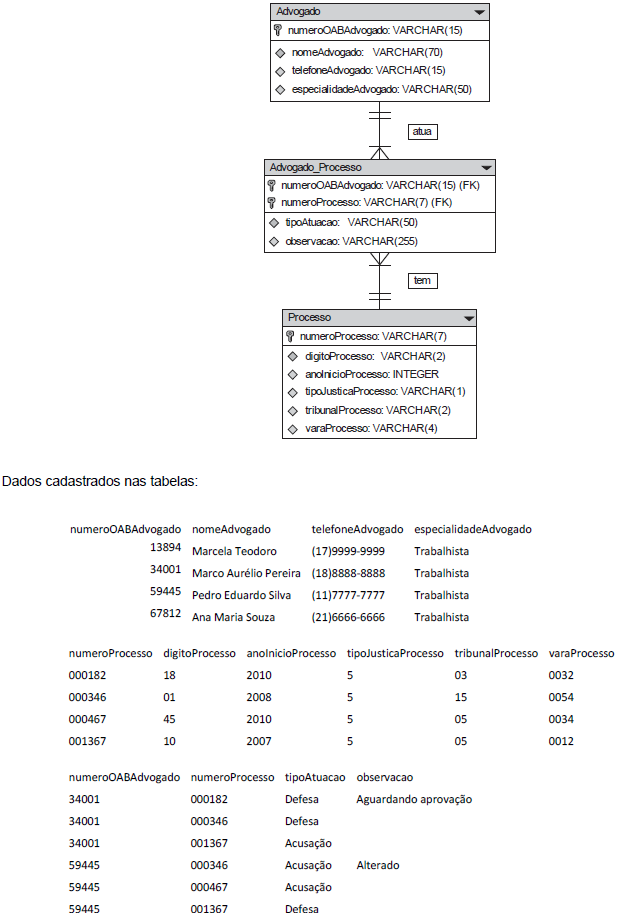
\includegraphics[width=0.9\linewidth]{figuras/819fcb79a990218cfea3}
%%\caption{}
%\label{fig:819fcb79a990218cfea3}
%\end{figure}
%
%\begin{checkboxes}
%\choice SELECT nomeAdvogado FROM advogado WHERE numeroOABAdvogado IS NOT(SELECT numeroOABAdvogado FROM advogado\underline{\hspace{0.1cm}}processo);
%\choice SELECT nomeAdvogado FROM advogado RIGHT JOIN advogado\underline{\hspace{0.1cm}}processo ON advogado.numeroOABAdvogado<>advogado\underline{\hspace{0.1cm}}processo.numeroOABAdvogado;
%\choice SELECT nomeAdvogado FROM advogado WHERE numeroOABAdvogado NOT IN (SELECT numeroOABAdvogado FROM advogado\underline{\hspace{0.1cm}}processo); 
%\choice SELECT DISTINCT nomeAdvogado FROM advogado JOIN advogado\underline{\hspace{0.1cm}}processo ON advogado.numeroOABAdvogado=advogado\underline{\hspace{0.1cm}}processo.numeroOABAdvogado;
%\choice SELECT DISTINCT nomeAdvogado FROM advogado WHERE nomeAdvogado NOT IN (SELECT nomeAdvogado FROM advogado\underline{\hspace{0.1cm}}processo);
%\end{checkboxes}
%
%\textbf{Gabarito:  SELECT nomeAdvogado FROM advogado WHERE numeroOABAdvogado NOT IN (SELECT numeroOABAdvogado FROM advogado\underline{\hspace{0.1cm}}processo); }

%\newpage

\question[0.5] Qual comando SQL retorna todos os clientes cuja cidade começa por qualquer caractere seguido por `uritiba'? 

\begin{checkboxes}
\CorrectChoice \begin{verbatim}select * from clientes where cidade like '_uritiba'\end{verbatim}
\choice  \begin{verbatim}select * from clientes where cidade like `%uritiba'\end{verbatim}
\choice \begin{verbatim}select * from clientes where cidade like `*uritiba'\end{verbatim}
\choice  \begin{verbatim}select * from clientes where cidade like `?uritiba'\end{verbatim}
\choice  \begin{verbatim}select * from clientes where cidade like `[ ]uritiba'\end{verbatim}
\end{checkboxes}

%\textbf{Gabarito: select * from clientes where cidade like '_uritiba'}

% \newpage

\question[0.5] Considere a seguinte tabela de um banco de dados relacional.

\vspace{5px}

\begin{center}
	Cliente (\underline{CPF}, Nome, Fone, End) 
\end{center} 

\vspace{10px}

O comando SQL para obter o Nome dos clientes, cujo campo Fone tenha o valor “nulo”, é:

\begin{checkboxes}
\choice \begin{verbatim}SELECT Nome (Fone NULL) FROM Cliente\end{verbatim}
\choice \begin{verbatim}SELECT Nome, Fone (NULL) FROM Cliente\end{verbatim}
\CorrectChoice \begin{verbatim}SELECT Nome FROM Cliente WHERE Fone IS NULL\end{verbatim}
\choice \begin{verbatim}SELECT Nome  FROM Cliente WHERE Fone = "NULL"\end{verbatim}
\choice \begin{verbatim}SELECT Nome FROM Cliente WHERE Fone LIKE "NULL"\end{verbatim}
\end{checkboxes}

%\textbf{Gabarito: SELECT Nome FROM Cliente WHERE Fone IS NULL}

% \question[0.5] Assinale a alternativa correta sobre fragmento de comando a seguir:

% \begin{center}
% \begin{verbatim}
% (select distinct nome_cliente from contas)
% intersect
% (select distinct nome_cliente from emprestimos) 
% \end{verbatim}
% \end{center}

% \begin{checkboxes}
% \choice Se um cliente possui conta mas não possui empréstimos no banco, aparecerá no resultado.
% \choice Se um cliente tem diversas contas e empréstimos no banco, aparecerá todas as repetições no resultado.
% \choice Se um cliente tem diversas contas e empréstimos no banco, não aparecerá no resultado.
% \choice Se um cliente tem diversas contas e empréstimos no banco, aparecerá somente uma vez no resultado.
% \choice Se um cliente não possui conta mas possui empréstimos no banco, aparecerá no resultado.
% \end{checkboxes}

%\textbf{Gabarito:  Se um cliente tem diversas contas e empréstimos no banco, aparecerá somente uma vez no resultado.}

% \question[0.5] A SQL disponibiliza funções de agregação para uso na interação com bancos de dados, conforme exemplificado nas perguntas a seguir.

% \begin{itemize}
% 	\choice Quantos são os ID relacionados à tabela de comissões (sem duplicidade)?	
% 	\choice Qual é a média das idades das pessoas que trabalham na empresa?
% \end{itemize}

% \newpage

% As instruções SQL que usam a função de agregação adequada para responder às duas questões são, respectivamente:

% \begin{checkboxes}
% 	\choice \begin{verbatim}SELECT COUNT(UNIQUE ID) AS TOTAL ON COMISSAO; e
% 	SELECT MED(IDADE) AS MEDIA_IDADES ON PESSOA;\end{verbatim}
% 	\choice \begin{verbatim}SELECT COUNT(DISTINCT ID) AS TOTAL ON COMISSAO; e
% 	SELECT AVG(IDADE) AS MEDIA_IDADES  ON PESSOA;\end{verbatim}
% 	\choice \begin{verbatim}SELECT COUNT(DISTINCT ID) AS TOTAL FROM COMISSAO; e 
% 	SELECT AVG(IDADE) AS MEDIA_IDADES FROM PESSOA;\end{verbatim}
% 	\choice \begin{verbatim}SELECT COUNT(UNIQUE ID) AS TOTAL  FROM COMISSAO; e
% 	SELECT MED(IDADE) AS MEDIA_IDADES FROM PESSOA;\end{verbatim}
% \end{checkboxes}

%\textbf{Gabarito: SELECT COUNT(DISTINCT ID) AS TOTAL FROM COMISSAO; e SELECT AVG(IDADE) AS MEDIA_IDADES FROM PESSOA;}


%\question[0.5] O operador EXCEPT de um comando SELECT da SQL do SGBD PostgreSQL tem por finalidade:
%
%\begin{checkboxes}
%\choice retornar as tuplas da primeira consulta que não estão na segunda.
%\choice retornar as tuplas da segunda consulta que não estão na primeira.
%\choice gerar uma exception em um comando SQL contido em uma trigger.
%\choice gerar uma exception em um comando SQL contido em uma stored procedure.
%\choice gerar uma exception em um comando SQL contido em uma stored procedure ou trigger.
%\end{checkboxes}
%
%\textbf{Gabarito: retornar as tuplas da primeira consulta que não estão na segunda.}

%\question[0.5] Escolha a sentença SQL que melhor responda à consulta “Listar a descrição da cor que não está presente em nenhum carro”: \label{cor}
%
%\begin{lstlisting}
%CREATE TABLE cor (
%	codigo INT NOT NULL,
%	descricao VARCHAR(100) NOT NULL,
%	PRIMARY KEY (codigo),
%	UNIQUE(descricao)	
%);
%
%CREATE TABLE carro (
%	codigo INT NOT NULL,
%	placar CHAR(7) NOT NULL,
%	cor INT NULL,
%	PRIMARY KEY (codigo),
%	UNIQUE (placa),
%	FOREIGN KEY (cor) REFERENCES cor (codigo)
%);
%\end{lstlisting}
%
%\begin{checkboxes}
%\choice SELECT cor.descricao FROM cor 
%LEFT JOIN carro c ON cor.codigo = c.cor 
%WHERE c.codigo IS NULL 
%\choice SELECT cor.descricao FROM cor 
%WHERE codigo NOT IN (SELECT codigo FROM carro) 
%\choice SELECT cor.descricao FROM cor 
%WHERE codigo NOT EXISTS (SELECT * FROM carro) 
%\choice SELECT cor.descricao FROM cor 
%WHERE NOT EXISTS (SELECT * FROM carro c 
%WHERE cor.codigo $<>$ c.cor)
%\end{checkboxes}
%
%\textbf{Gabarito: SELECT cor.descricao FROM cor 
%	LEFT JOIN carro c ON cor.codigo = c.cor 
%	WHERE c.codigo IS NULL } 

%\newpage

\newpage


\question[0.5] Considere as tabelas \textbf{nota} e \textbf{disciplina} abaixo:


\begin{table}[!htp]
	\caption{Tabela nota}
	\centering    	
	\begin{tabular}{|c|c|c|c|}
		\hline \textbf{seq}  &  \textbf{matricula}  &  \textbf{codDisciplina}  &   \textbf{valor} \\
\hline 1  &            1     &                  1   &              7.5 \\
\hline 1   &          2      &                 1      &            5 \\
\hline 2   &           1   &                    1     &             8 \\
\hline 2    &         2   &                     1      &            5 \\
\hline
\end{tabular}
\end{table}

\begin{table}[!htp]
	\caption{Tabela disciplina}
	\centering    	
	\begin{tabular}{|c|c|}
\hline \textbf{codDisciplina}  &    \textbf{nome} \\
\hline 1          &     Cálculo \\
\hline 2           &      Física \\
\hline 3           &    Química \\
\hline
\end{tabular}
\end{table}


O comando SQL que retorna as disciplinas que não possuem notas relacionadas é: 

\begin{checkboxes}
\CorrectChoice \begin{verbatim}SELECT nome from disciplina where disciplina.codDisciplina 
	not in (SELECT distinct(disciplina.codDisciplina) from nota, 
	disciplina where nota.codDisciplina = disciplina.codDisciplina)
\end{verbatim}
\choice  \begin{verbatim}SELECT nome from disciplina where disciplina.codDisciplina 
intersection 
SELECT distinct(disciplina.codDisciplina) from nota, disciplina 
where nota.codDisciplina = disciplina.codDisciplina
\end{verbatim}
\choice  \begin{verbatim}SELECT nome from disciplina where disciplina.codDisciplina in 
(SELECT distinct(disciplina.codDisciplina) from nota, disciplina 
where nota.codDisciplina = disciplina.codDisciplina) 
\end{verbatim}
\choice \begin{verbatim}SELECT nome, distinct(disciplina.codDisciplina) 
from nota, disciplina 
where nota.codDisciplina = disciplina.codDisciplina
\end{verbatim}
\choice \begin{verbatim}SELECT nome from disciplina where disciplina.codDisciplina union 
SELECT disciplina.nome from nota, disciplina 
where nota.codDisciplina = disciplina.codDisciplina
\end{verbatim}
\end{checkboxes}

%\textbf{Gabarito: SELECT nome from disciplina where disciplina.codDisciplina not in (SELECT distinct(disciplina.codDisciplina) from nota, disciplina where nota.codDisciplina = disciplina.codDisciplina)}

% \question[0.5] Quais são as marcações utilizadas no template do Spark?

% \begin{checkboxes}
% \choice \{ e \}
% \choice \{\{ e \}\}	
% \choice \$ e \$
% \choice \% e \%
% \choice $<\%$ e $\%>$
% \end{checkboxes}

%\textbf{Gabarito: \{\{ e \}\}}

% \question[0.5] Qual é a porta padrão do Spark?

% \begin{checkboxes}
% 	\choice 8080
% 	\choice 8086
% 	\choice 5432
% 	\choice 3306
% 	\choice 4567
% \end{checkboxes}

%\textbf{Gabarito: 4567}

%https://www.qconcursos.com/questoes-de-concursos/questoes/search?ano_publicacao=&area=&assunto=&caderno_id=&cargo=&codigo=78ecf2f4-9d&data=&data_comentario_texto=&disciplina=&escolaridade=&esfera=&instituto=&migalha=&minissimulado_id=&modalidade=&nao_resolvidas=&nivel_dificuldade=&order=questao_aplicada_em+desc&organizadora=&page=26&per_page=5&periodo_ate=&periodo_de=&possui_anotacoes=&possui_comentarios=&possui_comentarios_gerais=&possui_gabarito_comentado_texto_e_video=&product_id=1&prova=&q=select&resolvidas=&resolvidas_certas=&resolvidas_erradas=&sem_anuladas=&sem_anuladas_impressao=&sem_desatualizadas=&sem_desatualizadas_impressao=&sem_dos_meus_cadernos=&todas=on&url_solr=slave&user_id=128345&utf8=%E2%9C%93

\vspace{10px}

\question[0.5]  Um banco de dados relacional armazena duas tabelas, a tabela FUNCIONARIOS e a tabela DEPENDENTES, conforme apresentado abaixo. \label{questao_funcionario_dependente}

% \begin{figure}[!htp]
% \centering
% 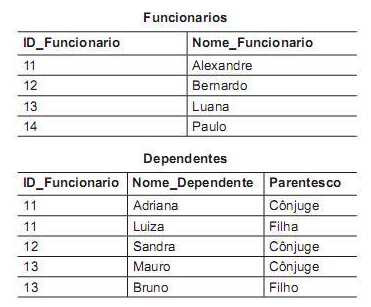
\includegraphics[width=0.5\linewidth]{figuras/funcionarios_dependentes}
% %\caption{Questão \ref{fig:funcionarios_dependentes}}
% \label{fig:funcionarios_dependentes}
% \end{figure}

\begin{table}[!ht]
\centering
\caption{Funcionarios}
\begin{tabular}{|c|c|}
\hline
\textbf{ID\_Funcionario} & \textbf{Nome\_Funcionario} \\ \hline
11                       & Alexandre                  \\ \hline
12                       & Benardo                    \\ \hline
13                       & Luana                      \\ \hline
14                       & Paulo                      \\ \hline
\end{tabular}
\end{table}


\begin{table}[!ht]
\centering
\caption{Dependentes}
\begin{tabular}{|c|c|c|}
\hline
\textbf{ID\_Funcionario} & \textbf{Nome\_Dependente} & \textbf{Parentesco} \\ \hline
11                       & Adriana                   & Cônjuge             \\ \hline
11                       & Luiza                     & Filha               \\ \hline
12                       & Sandra                    & Cônjuge             \\ \hline
13                       & Mauro                     & Cônjuge             \\ \hline
13                       & Bruno                     & Filho               \\ \hline
\end{tabular}
\end{table}

\vspace{10px}

Deseja-se elaborar uma consulta SQL para gerar um resultado com todos os funcionários e, para cada funcionário, o seu nome, o nome do dependente (ou null se não houver dependente) e o parentesco do dependente (ou null se não houver dependente). 

\newpage

Essa consulta será:
\begin{checkboxes}
	\choice \begin{verbatim}
	SELECT Nome_Funcionario, Nome_Dependente, Parentesco  
	FROM Funcionarios, Dependentes 
	WHERE Funcionarios.ID_Funcionario = Dependentes.ID_Funcionario;
	\end{verbatim}
\choice   
\begin{verbatim}
SELECT Nome_Funcionario, Nome_Dependente, Parentesco 
FROM Dependentes, Funcionarios 
WHERE Dependentes.ID_Funcionario = Funcionarios.ID_Funcionario;
\end{verbatim}
\choice  
\begin{verbatim}
SELECT Nome_Funcionario, Nome_Dependente, Parentesco 
FROM Funcionarios INNER JOIN Dependentes 
ON Funcionarios.ID_Funcionario = Dependentes.ID_Funcionario;
\end{verbatim}
\choice   
\begin{verbatim}
SELECT Nome_Funcionario, Nome_Dependente, Parentesco 
FROM Funcionarios RIGHT JOIN Dependentes 
ON Funcionarios.ID_Funcionario = Dependentes.ID_Funcionario;
\end{verbatim}
\CorrectChoice
\begin{verbatim}SELECT Nome_Funcionario, Nome_Dependente, Parentesco 
FROM Funcionarios LEFT JOIN Dependentes 
ON Funcionarios.ID_Funcionario = Dependentes.ID_Funcionario;
\end{verbatim}
\end{checkboxes}


% \question[0.5]  Observe a figura a seguir:
% \begin{figure}[!htp]
% \centering
% 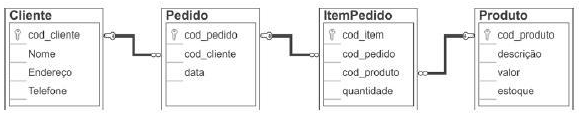
\includegraphics[width=1\linewidth]{figuras/pedido}
% %\caption{}
% \label{fig:pedido}
% \end{figure}

% A figura apresenta o modelo relacional de um Banco de Dados de um sistema de controle de estoque. Esse modelo possui as tabelas Cliente, Pedido, ItemPedido e Produto. Em uma leitura simplificada desse modelo tem-se que um cliente pode possuir vários pedidos, um pedido possui um ou vários itemPedidos e um item Pedido possui um produto e a quantidade desse produto.

% \vspace{10px}

% Assinale a alternativa que indique o comando SQL que, ao ser executado em um SGBD relacional baseado nesse modelo, retornará todos os nomes de clientes que fizeram pelo menos um pedido, a descrição do produto que o cliente comprou e a quantidade desse produto independente do pedido realizado.

% % \newpage

% \begin{checkboxes}
% \choice \begin{verbatim} SELECT Nome, descricao, sum (quantidade)
%  FROM Cliente INNER JOIN Pedido 
%  ON Cliente.cod_cliente = Pedido.cod_cliente
%  INNER JOIN ItemPedido 
%  ON Pedido.cod_pedido = ItemPedido.cod_pedido
%  INNER JOIN Produto 
%  ON ItemPedido.cod_produto = Produto.cod_produto
%  GROUP BY Nome, descricao\end{verbatim}
% \choice \begin{verbatim} SELECT Nome, descricao, count (quantidade)
%  FROM Cliente INNER JOIN Pedido 
%  ON Cliente.cod_cliente = Pedido.cod_cliente
%  INNER JOIN ItemPedido 
%  ON Pedido.cod_pedido = ItemPedido.cod_pedido
%  INNER JOIN Produto 
%  ON ItemPedido.cod_produto = Produto.cod_produto\end{verbatim}
%  \choice \begin{verbatim} SELECT Nome, descricao, count (quantidade)
%  FROM Cliente, Pedido, ItemPedido, Produto
%  WHERE Cliente.cod_cliente = Pedido.cod_cliente
%  AND Pedido.cod_pedido = ItemPedido.cod_pedido
%  AND ItemPedido.cod_produto = Produto.cod_produto\end{verbatim}
%  \choice \begin{verbatim} SELECT Nome, descricao, sum (quantidade)
%  FROM Cliente INNER JOIN Pedido 
%  ON Cliente.cod_cliente = Pedido.cod_cliente
%  INNER JOIN ItemPedido 
%  ON Pedido.cod_pedido = ItemPedido.cod_pedido
%  INNER JOIN Produto 
%  ON ItemPedido.cod_produto = Produto.cod_produto
%  GROUP BY quantidade\end{verbatim}
%  \choice \begin{verbatim} SELECT Nome, descricao, count (quantidade)
%  FROM Cliente, Pedido, ItemPedido, Produto
%  WHERE Cliente.cod_cliente = Pedido.cod_cliente
%  AND Pedido.cod_pedido = ItemPedido.cod_pedido
%  AND ItemPedido.cod_produto = Produto.cod_produto
%  GROUP BY cod_item, cod_prod\end{verbatim}
% \end{checkboxes}


% \question[0.5] Dada a instrução SQL: 

% \begin{verbatim}
% SELECT * FROM VENDEDOR 
% WHERE salario > (SELECT AVG(salario) FROM VENDEDOR);
% \end{verbatim}

% É correto afirmar que:
% \begin{checkboxes}
% \choice serão selecionados todos os registros da tabela VENDEDOR cujo conteúdo do campo "salario" seja maior que a soma dos salários de todos os vendedores.
% \choice  se trata de um exemplo de OUTER JOIN.
% \choice  serão selecionados todos os registros da tabela VENDEDOR cujo conteúdo do campo "salario" seja maior que a média dos salários de todos os vendedores.
% \choice  serão selecionados todos os registros da tabela VENDEDOR cujo conteúdo do campo "salario" seja maior que o número de vendedores cadastrados.
% \choice  se trata de um exemplo de INNER JOIN.
% \end{checkboxes}	

% \newpage

% \question[0.5] A expressão SQL correta é

% \begin{checkboxes}
% \choice \begin{verbatim}
% UPDATE table_name WHERE some_column=some_value 
% SET column1=value, column2=value2,...
% \end{verbatim}
% \choice \begin{verbatim}SELECT column_name(s) FROM table_name DISTINCT.
% \end{verbatim}
% \choice \begin{verbatim}SELECT column_name(s) FROM table_name LIKE pattern.\end{verbatim}
% \choice  \begin{verbatim}
% SELECT column_name(s) FROM table_name 
% WHERE column_name BETWEEN value1 AND value2.
% \end{verbatim}
% \choice \begin{verbatim}SELECT column_name(s) TOP number|percent FROM table_name.
% \end{verbatim}
% \end{checkboxes}

\vspace{10px}

\question[0.5] A estrutura de controle Iteração pode ser utilizada em PL/SQL com os comandos

\begin{checkboxes}
\choice LOOP, CASE-LOOP, WHILE-LOOP e FOR-LOOP.
\choice LOOP, CASE-LOOP e WHILE-LOOP.
\choice LOOP, CASE-LOOP e FOR-LOOP.
\choice CASE-LOOP, WHILE-LOOP e FOR-LOOP.
\CorrectChoice LOOP, WHILE-LOOP e FOR-LOOP.
\end{checkboxes}


% \question[0.5] Para obter todas as linhas da tabela B, o comando SELECT deverá utilizar na sequência um JOIN entre as tabelas A e B do tipo:

% \begin{checkboxes}
% \choice CROSS JOIN.
% \choice INNER JOIN.
% \choice FULL JOIN.
% \choice RIGHT JOIN.
% \choice LEFT JOIN.
% \end{checkboxes}

\newpage

\question[0.5] Considere o seguinte comando para a criação de um \textbf{trigger} em SGBD relacional:

\begin{verbatim}
CREATE TRIGGER T AFTER UPDATE ON R
\end{verbatim}

Esse comando tem como efeito a criação de um trigger chamado:
\begin{checkboxes}
\choice R, somente após a iniciação geral do sistema.
\choice R, somente após uma atualização da estrutura da tabela T.
\choice R, somente após a atualização de algum registro da tabela T.
\CorrectChoice T, somente após a atualização de algum registro da tabela R.
\choice T, somente após atualização de todos os registros da tabela R.
\end{checkboxes}


% \question[0.5] Considere: 

% \begin{enumerate}
% 	\choice Retorna linhas quando houver pelo menos uma correspondência entre duas tabelas. 
% 	\choice Operador usado para combinar o resultado do conjunto de duas ou mais instruções SELECT. 
% 	\choice Operador usado em uma cláusula WHERE para pesquisar um padrão específico em uma coluna. 
% \end{enumerate}

% 1, 2 e 3 correspondem em SQL, respectivamente, a:


% \begin{checkboxes}
% 	\choice SELECT, UNIQUE e BETWEEN.
% 	\choice INNER JOIN, JOIN e DISTINCT.
% 	\choice LEFT JOIN, UNIQUE e LIKE.
% 	\choice SELECT, JOIN e BETWEEN.
% 	\choice INNER JOIN, UNION e LIKE.
% \end{checkboxes}


% \question[0.5] Considere a tabela abaixo:

% \begin{lstlisting}[frame=single]
% 			func(nome, salario);
% \end{lstlisting}

% O comando SQL que deve ser usado para obter o maior valor da coluna \textbf{SALARIO} é:

% \begin{checkboxes}
% \choice \begin{verbatim}Select salario as max from func\end{verbatim}
% \choice \begin{verbatim}Select salario from func where salario = Max\end{verbatim}
% \choice \begin{verbatim}Select max(salario) from func \end{verbatim}
% \choice \begin{verbatim}Select salario from func where salario >= salario \end{verbatim}
% \choice \begin{verbatim}Select max from func(salario)\end{verbatim}
% \end{checkboxes}

\question[0.5] A seção do bloco PL/SQL executável e dentro da qual ficam instruções procedimentais e SQL é a:

\begin{checkboxes}
\choice EXCEPTION.
\choice SELECTION.
\choice EXECUTE.
\choice DECLARE.
\CorrectChoice BEGIN.
\end{checkboxes}

% \question[0.5] Considere a tabela \textbf{Pessoa} abaixo: 
%
%\begin{figure}[!htp]
%	\centering
%	\includegraphics[width=0.7\linewidth]{figuras/distinct}
%	\label{fig:distinct}
%\end{figure}

% \vspace{8px}

%\begin{table}[!htp]
%%	\centering
% \begin{tabular}{|c|c|c|c|c|}
% 	\hline 
% 	\textbf{id} & \textbf{Sobrenome} & \textbf{Nome} & \textbf{Endereço} & \textbf{Cidade} \\ \hline  
% 	1 & Tulio & Nelson & Rua Sete & Santos \\ \hline  
% 	2 & Madeira & Carla & Av. Quadrante & Santos  \\ \hline
% 	3 & Pereira & Patricia & Praça Julio & Campinas \\ \hline  	
% \end{tabular} 
%\end{table}

% \vspace{8px}

% A expressão \textbf{SELECT DISTINCT Cidade FROM Pessoa}, terá como resultado:

% \begin{checkboxes}
% 	\choice Santos.
% 	\choice Santos e Santos.
% 	\choice Santos e Campinas.
% 	\choice Campinas.
% 	\choice Santos, Santos e Campinas.
% \end{checkboxes}


\question[0.5] Dado um banco de dados relacional formado pela tabela abaixo:

\begin{figure}[!htp]
	\centering
	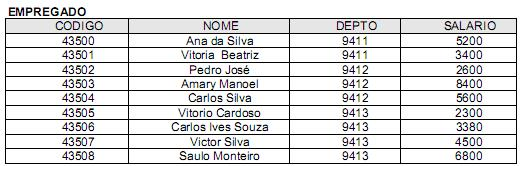
\includegraphics[width=0.9\linewidth]{figuras/count_avg}
	%\caption{}
	\label{fig:count_avg}
\end{figure}



O comando SQL que lista o total de empregados por departamento e a média salarial por departamento é dado por:

\begin{checkboxes}
	\CorrectChoice \begin{verbatim}
	SELECT DEPTO, COUNT(*), AVG(SALARIO) FROM EMPREGADO 
	GROUP BY DEPTO
	\end{verbatim}
	\choice \begin{verbatim}
	SELECT COUNT(NOME), AVERAGY(SALARIO) 
	GROUP DEPTO
	\end{verbatim}
	\choice \begin{verbatim}
	SELECT TOTAL(CODIGO) AND AVERAGY(SALARIO) 
	AGROUPED DEPTO
	\end{verbatim} 
	\choice \begin{verbatim}
	SELECT TOT (SALARIO), AVG(SALARIO) ORDER BY DEPTO
	\end{verbatim}
\end{checkboxes}

% \question[0.5] No Java, a classe \textit{DriverManager} fornece os serviços básicos para gerenciamento de drivers JDBC. Quais três argumentos normalmente são passados como parâmetros em seu método \textit{getConnection}? 

% \begin{checkboxes}
% \choice String url, String user e String password.
% \choice String url, String port e String database.
% \choice String url, String user e String database. 
% \choice String user, String port e String database.
% \choice String user, String password e String database. 
% \end{checkboxes}

% \question[0.5] O método a seguir está presente em uma classe de acesso a dados (DAO) de uma aplicação construída com Java utilizando JDBC. 


%\begin{figure}[!htp]
%\centering
%\includegraphics[width=0.7\linewidth]{figuras/dao}
%%\caption{}
%\label{fig:dao}
%\end{figure}


% \begin{lstlisting}
% public int salvarCliente(int varId, String varNome, double varRenda){
% 	try{
% 		I
% 		....
% 		st.setInt(1, varId);
% 		st.setString(2, varNome);
% 		st.setDouble(3, varRenda);
% 		retorno = st.executeUpdate();
% 	} catch (SQLException e){
% 		retorno = -1;
% 	}
% 	return retorno;
% }
% \end{lstlisting}


% Considere que:

% \begin{itemize}
% 	\choice a variável \textbf{conn} é da interface \textbf{Connection}, \textbf{st} é da interface \textbf{PreparedStatement} e retorno é uma variável do tipo int, todas declaradas e inicializadas anteriormente.
% 	\choice uma conexão com um banco de dados que contém a tabela cliente foi estabelecida com sucesso e em condições ideais.
% 	\choice a tabela cliente possui os campos abaixo:
% 	\begin{itemize}
% 		\choice id - inteiro, não nulo, chave primária
% 		\choice nome - cadeia de caracteres
% 		\choice renda - real
% 	\end{itemize}
% \end{itemize}

% \newpage

% Nestas condições, para que o método esteja correto, a lacuna I deve ser preenchida com a instrução:

% \begin{checkboxes}
% \choice  st = conn.prepareStatement("insert into cliente (id, nome, renda) values (?, ?, ?)");
% \choice 
%  st = conn.prepareStatement("insert into cliente (id, nome, renda) values (varId, varNome, varRenda)"); 
% \choice  st = conn.preparedStatement("insert into cliente (id, nome, renda) values (?, ?, ?)"); 
% \choice  st = conn.prepareStatement("insert into cliente(id,nome,renda) values( "+varId+","+varNome+" ,'"+varRenda+"')"); 
% \choice  st = conn.executeStatement("insert into cliente values ( '" + varId + "', " + varNome + " , '" + varRenda + "')"); 
% \end{checkboxes}

% \question[0.5] Na API JDBC (Java Database Connectivity), o valor retornado pelo método executeQuery da interface java.sql.Statement é uma referência a uma instância da classe:

% \begin{checkboxes}
% \choice  ResultList;
% \choice  ResultMap;
% \choice  ResultCollection;
% \choice  RowSet;
% \choice  ResultSet. 
% \end{checkboxes}

% \question[0.5] Sobre este método é correto afirmar que:

%\begin{figure}[!htp]
%	\centering
%	\includegraphics[width=0.5\linewidth]{figuras/conectar}
%	%\caption{}
%	\label{fig:conectar}
%\end{figure}

% \begin{lstlisting}
% public int conectar(String a, String b, String c, String d){
% 	try{
% 		Class.forName(a);
% 		x = DriverManager.getConnection(b, c, d);
% 		y = x.createStatement();
% 		return 1;
% 	} catch (ClassNotFoundException ex){
% 		return 2;
% 	} catch (SQLException ex1){
% 		return 3;
% 	}
% }
% \end{lstlisting}


% \begin{checkboxes}
% 	\choice o parâmetro \textbf{d} refere-se ao endereço do banco de dados. 
% 	\choice \textbf{x} é um objeto da interface SQLConnection. 
% 	\choice \textbf{y} é um objeto da interface PreparedStatement. 
% 	\choice o parâmetro \textbf{b} refere-se ao nome do usuário do banco de dados.
% 	\choice o parâmetro \textbf{a} refere-se ao driver JDBC.
% \end{checkboxes}	

% \newpage

% \question[0.5] Analise o código a seguir.

%\begin{figure}[!htp]
%	\centering
%	\includegraphics[width=0.5\linewidth]{figuras/dao2.png}
%	%\caption{}
%	\label{fig:dao2}
%\end{figure}

% \begin{lstlisting}
% public class Dao{
% 	public int metodoA(String v){
% 		int x = 0;
% 		try {
% 			Class.forName("com.mysql.jdbc.Driver");
% 			Connection con = DriverManager.getConnection("jdbc:mysql://localhost:3306/controle", "root", "x");
% 			Statement st = con.createStatement();
% 			x = st.executeUpdate(v);
% 			return x;
% 		} catch (ClassNotFoundException ex){
% 			return x;
% 		} catch (Exception ex1){
% 			return x;
% 		}
% 	}
% }
% \end{lstlisting}

% Para que o metodoA execute a operação desejada, na chamada ao método executeUpdate é necessário que ele receba como parâmetro uma instrução DML SQL

% \begin{checkboxes}
% \choice update, apenas.
% \choice insert, update, delete ou select.
% \choice insert, update ou delete, apenas.
% \choice insert, apenas.
% \choice update ou select, apenas.
% \end{checkboxes}

% \question[0.5] Em uma conexão JDBC com um banco de dados utilizando as classes e interfaces do pacote java.sql, o método para o qual se passa o driver de conexão é o

% \begin{checkboxes}
% \choice \textit{setDriver}, da classe \textit{Connection}.
% \choice \textit{setDriver}, da classe \textit{Class}.
% \choice \textit{forName}, da classe \textit{Connection}.
% \choice \textit{driverManager}, da classe \textit{Class}.
% \choice \textit{forName}, da classe \textit{Class}.
% \end{checkboxes}

% \newpage


% \question[0.5] Nas classes, nas quais estes métodos se encontram, foram importados todos os recursos necessários para a execução. O banco de dados, a tabela e o driver JDBC existem e funcionam corretamente. 

% %\begin{figure}[!htp]
% %\centering
% %\includegraphics[width=0.9\linewidth]{figuras/metodo1}
% %%\caption{}
% %\label{fig:metodo1}
% %\end{figure}

% \vspace{12px}

% \textbf{Método 1}

% \vspace{12px}


% \begin{lstlisting}
% public int inserir(int varId, String varNome, double varRenda){
% 	int retorno;
% 	try{
% 		Class.forName("com.mysql.jdbc.Driver");
% 		Connection conn = DriverManager.getConnection("jdbc:mysql://localhost:3306/bd007", "root", "1234");
% 		PrepareStatement st = conn.prepareStatement("insert into cliente (id, nome, renda) values (?,?,?);");
% 		st.setInt(1, varId);
% 		st.setString(2, varNome);
% 		st.setDouble(3, varRenda);
% 		retorno = st.executeUpdate();
% 	} catch (ClassNotFoundException ex){
% 		retorno = 0;		
% 	} catch (SQLException ex1){
% 		retorno = 0;
% 	}
% 	return retorno;
% }
% \end{lstlisting}


% \vspace{12px}

% \textbf{Método 2}

% \vspace{12px}

% \begin{lstlisting}
% public int inserir (int varId, String varNome, double varRenda){
% 	int retorno;
% 	try{
% 		Class.forName("com.mysql.jdbc.Driver");
% 		Connection conn =  DriverManager.getConnection("jdbc:mysql://localhost:3306/bd007","root","1234");
% 		Statement st = conn.createStatement();
% 		retorno = st.executeUpdate("insert into cliente values ('"+varId+"', '"+varNome+"', "+varRenda+")");
% 	} catch (ClassNotFoundException ex){
% 		retorno = 0;		
% 	} catch (SQLException ex1){
% 		retorno = 0;
% 	}
% 	return retorno;
% }
% \end{lstlisting}

%\begin{figure}[!htp]
%	\centering
%	\includegraphics[width=0.9\linewidth]{figuras/metodo2}
%%	\caption{}
%	\label{fig:metodo2}
%\end{figure}

% \newpage

% É correto afirmar que:

% \begin{checkboxes}
% \choice o Método 1 está incorreto, pois o método executeUpdate da interface PreparedStatement precisa receber como parâmetro a instrução SQL insert a ser executada.
% \choice o Método 2 está incorreto, pois o método executeUpdate da interface Statement não pode receber parâmetros. A instrução insert passada como parâmetro nesse método deveria ser passada como parâmetro para o método createStatement da interface Connection.
% \choice ambos os métodos estão corretos e executam a mesma operação, apresentando os mesmos resultados.
% \choice ambos os métodos estão incorretos, pois o método presente tanto na interface Statement como na interface PreparedStatement para incluir dados na tabela do banco de dados é o método executeInsert e não executeUpdate .
% \choice o Método 1 está incorreto, pois a instrução insert passada como parâmetro para o método PreparedStatement da interface Connection está incompleta. No lugar dos pontos de interrogação devem ser colocados os valores que devem ser incluídos nos campos id , nome e renda da tabela.	
% \end{checkboxes}
	
% \question[0.5] A utilização de JDBC, em um programa Java, inicia com a indicação do pacote que contém a JDBC API pela declaração: 

% \begin{checkboxes}
% \choice import java.awt.*;
% \choice import java.util.*;
% \choice import java.sql.*;
% \choice import java.swing.*;
% \choice import java.jdbc.*;	
% \end{checkboxes}

% \question[0.5] Em uma aplicação Java, se o carregador de classes não conseguir localizar a classe do driver de banco de dados para uma conexão JDBC, é lançada a exceção:

% \begin{checkboxes}
% \choice java.lang.ClassNotFoundException.
% \choice java.io.FileNotFoundException.
% \choice java.lang.SecurityException.
% \choice java.io.IOException.
% \choice java.util.InputMismatchException.
% \end{checkboxes}


% \question[0.5] Analise as linhas a seguir presentes em um programa Java que não apresenta erros. 

% \begin{itemize} 
% \choice a = DriverManager.getConnection("jdbc:postgresql://localhost/database", "username", "password");
% \choice b = a.createStatement(); 
% \choice c = b.executeQuery("select * from cliente where id = "+ valor +""); 
% \end{itemize}

% Considere que os objetos a, b e c são de interfaces contidas no pacote java.sql. Pode-se concluir que esses objetos são, respectivamente, das interfaces: 

% \begin{checkboxes}
% \choice Connection, SessionStatement e Result. 
% \choice DriverManager, PreparedStatement e RecordSet. 
% \choice ConnectionStatement, PreparedStatement e RecordSet.
% \choice Connection, Statement e ResultSet.
% \choice DaoConnection, Statement e ResultSet.
% \end{checkboxes}

% \question[0.5] A diferença básica dos conceitos de \textit{trigger} e \textit{stored procedure} é que, respectivamente:

% \begin{checkboxes}
% \choice são executadas de acordo com um evento, mas não são inclusas no banco de dados.
% \choice  é executada de acordo com um evento; é chamada para ser executada e são inclusas no banco de dados.
% \choice  são executadas após serem chamadas, porém a primeira não é inclusa no banco de dados.
% \choice são executadas após serem chamadas, porém a segunda não é inclusa no banco de dados.
% \choice  é chamada para ser executada; é executada de acordo com um evento e não são inclusas no banco de dados.
% \end{checkboxes}

\question[0.5] A expressão SQL correta é

\begin{checkboxes}
\item \begin{verbatim}UPDATE table_name 
WHERE some_column=some_value 
SET column1=value, column2=value2,...
\end{verbatim}
\item \begin{verbatim}SELECT column_name(s) FROM table_name DISTINCT.
\end{verbatim}
\item \begin{verbatim}SELECT column_name(s) FROM table_name LIKE pattern.\end{verbatim}
\CorrectChoice \begin{verbatim}SELECT column_name(s) FROM table_name 
WHERE column_name BETWEEN value1 AND value2.
\end{verbatim}
\item \begin{verbatim}SELECT column_name(s) TOP number|percent FROM table_name.
\end{verbatim}
\end{checkboxes}


\question[0.5]  Na linguagem SQL, são procedimentos executados implicitamente quando ocorre determinada ação do usuário, tal qual, uma modificação de uma tabela:

\begin{checkboxes}
\choice Inserts.
\choice Queries.
\choice Views.
\CorrectChoice Triggers.
\choice Selects.
\end{checkboxes}


% \question[0.5]  Com relação ao uso da SQL na manipulação de dados, caso se queira eliminar linhas repetidas do conjunto resultado, deve-se utilizar a palavra-chave DISTINCT, da seguinte forma:

% \begin{checkboxes}
% \choice \begin{verbatim}SELECT DISTINCT {colunas} FROM {tabelas}\end{verbatim}
% \choice \begin{verbatim}DISTINCT SELECT {colunas} FROM {tabelas}\end{verbatim}
% \choice \begin{verbatim}SELECT {colunas} FROM {tabelas} DISTINCT\end{verbatim}
% \choice \begin{verbatim}SELECT FROM {tabelas} DISTINCT {colunas}\end{verbatim}
% \end{checkboxes}

\question[0.5] A instrução SQL em PostgreSQL abaixo está mal formulada. 

\vspace{10px}

\begin{verbatim}
CREATE VIEW vista AS SELECT `HelloWorld';    
\end{verbatim}

\vspace{10px}

Isto aconteceu, porque:

\begin{checkboxes}
\choice a criação de uma visualização requer a utilização da cláusula WHERE para a restrição dos dados.
\choice não é possível criar uma VIEW sem a identificação do tipo de dado e sem a determinação da quantidade de registros selecionados.
\choice o comando CREATE VIEW deve utilizar a cláusula FROM para o nome da tabela.
\choice a criação de uma visualização ( VIEW ) requer a definição de um gatilho ( trigger ) correspondente ao nome da coluna.
\CorrectChoice  por padrão, o tipo de dado será considerado indefinido (unknown) e a coluna irá utilizar o nome padrão ?column?.
\end{checkboxes}

\newpage

 \question[0.5] Em PostgreSQL, a palavra chave utilizada na clausula CREATE TABLE para indicar que uma tabela herda os atributos de uma outra tabela e:

 \begin{checkboxes}
 \choice EXTENDS
 \CorrectChoice INHERITS.
 \choice IMPLEMENTS.
\choice REFERENCES.
\choice CONSTRAINT. 
\end{checkboxes}

% \question[0.5] Considerando o banco de dados PostgreSQL 8.4, assinale a alternativa que representa o comando utilizado para efetuar backup do banco de dados.
% \begin{checkboxes}
% \choice pg\underline{\hspace{0.3cm}}backup
% \choice pg\underline{\hspace{0.3cm}}dump
% \choice postgrebkp
% \choice pg\underline{\hspace{0.3cm}}save
% \choice pg\underline{\hspace{0.3cm}}restore
% \end{checkboxes}

\question[0.5] No PostgreSQL, para remover o valor padrão de uma coluna chamada preco em uma tabela chamada produto de um banco de dados ativo, em condições ideais, utiliza-se a instrução
\begin{checkboxes}
\CorrectChoice \begin{verbatim}ALTER TABLE produto 
ALTER COLUMN preco DROP DEFAULT;
\end{verbatim}
\choice \begin{verbatim}ALTER COLUMN preco FROM produto 
DROP DEFAULT ON;\end{verbatim}
\choice \begin{verbatim}MODIFY COLUMN preco FROM produto 
DROP DEFAULT;\end{verbatim}
\choice \begin{verbatim}ALTER COLUMN preco FROM produto 
REMOVE DEFAULT;\end{verbatim}
\choice \begin{verbatim}ALTER TABLE produto MODIFY COLUMN 
preco DROP DEFAULT ON;\end{verbatim}
\end{checkboxes}

% \question[0.5] No PostgreSQL, é possível atualizar um campo do banco de dados usando-se o comando a seguir. 

% \begin{verbatim}
% UPDATE a,b SET a.id=b.id WHERE a.f2 = b.f2;
% \end{verbatim}

% \begin{checkboxes}
% 	\choice Certo
% 	\choice Errado
% \end{checkboxes}

% \newpage


%\question[0.5] Uma tabela chamada tribunais de um banco de dados chamado TRF do PostgreSQL possui os seguintes campos: 

%\begin{figure}[!htp]
%\centering
%\includegraphics[width=0.7\linewidth]{figuras/imagem-003}
%%\caption{}
%\label{fig:imagem-003}
%\end{figure}

%\begin{verbatim}
%No_Regiao integer
%Nome_Tribunal character varying(100),
%ID_Tribunal character varying(10) not null primary key 
%\end{verbatim}

%Nesta tabela estão cadastrados os seguintes dados:

%\begin{table}[!htp]
%	\centering
%	\caption{}
%	\label{}
%	\begin{tabular}{|l|l|l|}
	%	\hline
	%	No\_Regiao & Nome\_Tribunal                 & ID\_Tribunal \\ \hline
	%	1          & Tribunal Regional da 1ª Região & TRF1         \\ \hline
	%	2          & Tribunal Regional da 2ª Região & TRF2         \\ \hline
	%	3          & Tribunal Regional da 3ª Região & TRF3         \\ \hline
	%	4          & Tribunal Regional da 4ª Região & TRF4         \\ \hline
%	\end{tabular}
%\end%{table}

%No PostgreSQL, para exibir os registros cujos valores contidos no campo No\underline{\hspace{0.3cm}}Regiao estejam entre 1 e 3, excluindo-se da exibição aqueles cujo conteúdo do campo ID\underline{\hspace{0.3cm}}Tribunal contenha os valores TRF2 ou TRF3, utiliza-se a instrução:

%\begin{checkboxes}

%\choice \begin{verbatim}SELECT * FROM "TRF".tribunais 
%WHERE ("No_Regiao" BETWEEN 1 AND 3) 
%AND NOT "ID_Tribunal" EQUALS ('TRF2' OR 'TRF3');
%\end{verbatim}
 
%\choice \begin{verbatim}SELECT * FROM "TRF".tribunais 
%WHERE ("No_Regiao" BETWEEN 1 AND 3) 
%AND "ID_Tribunal" IN NOT('TRF2','TRF3');\end{verbatim}
 
%\choice  \begin{verbatim}SELECT * FROM tribunais 
%WHERE (No_Regiao BETWEEN 1 AND 3) 
%AND NOT ID_Tribunal='TRF2' OR ID_Tribunal='TRF3';\end{verbatim}
 
% \choice  \begin{verbatim}SELECT * FROM "TRF".tribunais 
% WHERE ("No_Regiao" BETWEEN 1 AND 3) 
% AND NOT "ID_Tribunal" IN ('TRF2','TRF3');\end{verbatim}
 
% \choice  \begin{verbatim}SELECT * FROM tribunais 
% WHERE (1<No_Regiao<3) AND NOT ID_Tribunal IN ('TRF2','TRF3');\end{verbatim}
%\end{checkboxes}

\question[0.5] Considere o trecho em PostgreSQL abaixo. 

%\begin{figure}[!htp]
%\centering
%\includegraphics[width=1\linewidth]{figuras/insert_products}
%%\caption{}
%\label{fig:insert_products}
%\end{figure}
\begin{verbatim}
INSERT INTO products (product_no, name, price) VALUES 
	(1, `Cheese', 9.99), 
	(2, `Bread', 1.99), 
	(3, `Milk', 2.99);
\end{verbatim}
Considerando a existência prévia da tabela \textit{products} contendo as colunas \textit{product\underline{\hspace{0.2cm}}no}, \textit{name} e \textit{price}, e desconsiderando os tipos de dados, esse trecho irá resultar:

\begin{checkboxes}
\choice na adição de 3 novas colunas na tabela \textit{products}.
\CorrectChoice na adição de 3 novas linhas na tabela \textit{products}.
\choice em erro, pois não é possível múltiplas inserções em um único comando SQL.
\choice em erro, pois para se realizar múltiplas inserções é necessário a utilização da cláusula SELECT.
\choice em erro, pois múltiplas inserções são possíveis somente com a utilização de colchetes para a limitação dos registros.
\end{checkboxes}


% \question[0.5] Em um SGBD, se ocupa respectivamente de alteração de tabela (ex. Alter Table), atualização de uma linha de tabela (ex. Update) e exclusão de visão (ex. Drop View), a:
% \begin{checkboxes}
% \choice DDL, DML e DDL.
% \choice DDL, DDL e DML.
% \choice DML, DDL e DML.
% \choice DML, DML e DDL.
% \choice DDL, DML e DML.
% \end{checkboxes}


% \question[0.5] Em PL/SQL, COALESCE (expr1, expr2) é equivalente a:

% \begin{checkboxes}
% \choice CASE WHEN expr1 = expr2 AND expr1 IS NOT NULL END
% \choice SUBSTR (expr1, expr2)
% \choice MAX ( expr1, expr2)
% \choice  CASE WHEN expr1 IS NOT NULL THEN expr1 ELSE expr2 END
% \choice WHERE expr1 IN expr2
% \end{checkboxes}


% \question[0.5] Analise o seguinte comando SQL: 

% \begin{verbatim}
% SELECT COUNT(....I... ) FROM Clientes; 
% \end{verbatim}

% Para que o resultado seja a contagem de linhas que possuam valores não repetidos para a coluna ID, a lacuna I deve ser preenchida com :

% \begin{checkboxes}
% \choice COALESCE(ID) 
% \choice  *
% \choice  UNIQUE ID
% \choice  DISTINCT ID
% \choice  NOT COLIDE ID
% \end{checkboxes}

% \question[0.5] Que comando SQL cria uma visão?
% \begin{checkboxes}
% \choice NEW VISION
% \choice NEW VIEW
% \choice INSERT VISION
% \choice CREATE VIEW
% \choice CREATE VISION
% \end{checkboxes}

\end{questions}

\end{document}